\section{Desarrollo protocolo de control in-band}
\label{sec:bofussDEV}


En esta sección se va a explicar la implementación realizada del protocolo IoTorii en el \textit{software switch} \gls{bofus}. Dado que el trabajo de implementación ha sido bastante extenso, dado que había que discernir que parte de la implementación del control in-band podía ser aprovechada, se ha decidido generar un documento anexo \cite{davidBOFUSS} aparte de la memoria, donde se explique a bajo nivel las modificaciones realizadas. Todo el código se puede encontrar indicado en la Sección \ref{sec:estadoArte_github}. \\
\\
En la Figura \ref{fig:WIN-BOFUSS}, se puede apreciar la secuencia lógica que se ha llevado a cabo para la implementación del protocolo IoTorii en el software switch. En adelante se podrá encontrar el termino \texttt{win-BOFUSS}, el cual hará referencia a la implementación del protocolo IoTorii en la implementación de in-band del \gls{bofus}, conocida como \texttt{in-BOFUSS}, por lo que para añadirle la condición de \textit{wireless} se ha apodado como \texttt{win-BOFUSS}, del inglés \textit{\textbf{w}ireless \textbf{in}-band \textbf{B}asic \textbf{O}pen\textbf{F}low \textbf{U}serspace \textbf{S}oftware \textbf{S}witch}. En primer lugar, se han detectado todas las modificaciones realizadas anteriormente en la implementación del control in-band llevada a cabo por Boby N. Constantin \cite{constantin2020desarrollo}, y posteriormente se han clasificado en tres bloques funcionales: (1) Modificaciones del puerto local del ofprotocol, (2) Implementación de la  lógica de control del modo in-band, (3) Implementación del protocolo Amaru.\\
\\
Una vez se han identificado y se han clasificado todas las modificaciones realizadas sobre el switch \gls{bofus}, se va a pasar a la siguiente etapa, en la cual se va a ir módulo por módulo analizando y decidiendo si las modificacioens de cada módulo pueden ser aprovechadas en la implementación del \texttt{win-BOFUSS}. La primera modificación hacía referencia a un error en el tamaño del identificador del puerto local en el bloque de ofprotocol, tienendo que ser aplicado a 16 bits. Durante el desarrollo del \texttt{in-BOFUSS}, identificó que la lógica encargada de implementar el funcionamiento in-band del software-switch no se ejecutaba de manera adecuada. Se descubrió que este problema se debía a una discrepancia en el tamaño del identificador del puerto local, lo cual impedía que los datos correspondientes a dicho puerto fueran almacenados correctamente en la estructura utilizada por el módulo ofprotocol para almacenar los datos de los puertos del switch \gls{bofus}. Dado que dichas modificaciones son necesarias para el desarrollo del \texttt{win-BOFUSS}, se han reaprovechado.\\
\\
Una vez reaprovechado dicho módulo de modificaciones, se ha seguido por el siguiente módulo el cual hace referencia a la implementación del control in-band del \textit{software switch}. En la implementación del \texttt{in-BOFUSS}, se detectó que el switch era incapaz de instalar reglas en las \textit{flow tables} de forma automatica en aras de mandar el tráfico de control OpenFlow por los puertos indicados. Esto se debía a que los mensajes encargados de instalar las reglas conocidos como \texttt{FLOW\_MOD}, generados de forma local, estaban siendo marcados como erróneos dado que estaban siendo mal generados, y por ello, el binario ofdatapath no podía instalar dichas reglas.\\
\\
Más específicamente, se ha observado que la estructura de matches no se genera de manera correcta, lo cual impide que el módulo ofdatapath pueda extraer los matches e implementar adecuadamente las reglas en su tabla de flujos. El objetivo de las modificaciones es permitir que el módulo ofprotocol sea capaz de crear mensajes \texttt{FLOW\_MOD} que añadan, modifiquen o eliminen las reglas necesarias para el funcionamiento en modo in-band. Las principales modificaciones implementadas por mi compañero fueron las siguientes:

\begin{itemize}
    \item Función \texttt{make\_flow\_mod()} del archivo \texttt{ofp.c}: Se ha corregido la generación de la estructura de matches para el paquete \texttt{FLOW\_MOD} y se han completado los campos requeridos de los paquetes \texttt{FLOW\_MOD}. Para asegurar una generación precisa de la estructura de match, se ha implementado la función \texttt{create\_ofl\_match\_UAH()}.

    \item Función \texttt{make\_add\_flow()} del archivo \texttt{ofp.c}: Se ha introducido la creación de un paquete \texttt{FLOW\_MOD} de tipo DROP, que instala una regla para descartar el flujo especificado en la estructura de match cuando el tamaño de las acciones es igual a 0. En caso contrario, se genera un \texttt{FLOW\_MOD} normal.

    \item Función \texttt{make\_add\_simple\_flow()} del archivo \texttt{ofp.c}: Se ha modificado para que cree un paquete \texttt{FLOW\_MOD} que instale una regla para encaminar el tráfico, identificado por los campos de match, hacia un puerto específico. Si el puerto de salida es 0, se crea un \texttt{FLOW\_MOD} del tipo DROP, es decir, una regla para descartar los paquetes correspondientes al tráfico caracterizado por los campos de match.
\end{itemize}

Tras realizar las modificaciones pertinentes en los mecanismos y lograr que los mensajes \texttt{FLOW\_MOD} instalaran correctamente las reglas, se evidenció un inconveniente en la lógica del bloque ofprotocol encargado de analizar los mensajes \texttt{PACKET\_IN} antes de enviarlos al controlador. Dicha lógica tiene como finalidad extraer la información necesaria del paquete encapsulado en el mensaje \texttt{PACKET\_IN}, con el propósito de crear las reglas que permiten configurar el control in-band. Se constató que no se extraía adecuadamente el puerto de entrada del paquete encapsulado, lo que imposibilitaba la instalación de las reglas que dependían de esta información.\\
\\
A raíz de ello, se procedió a efectuar las modificaciones necesarias para obtener de forma precisa el puerto de entrada. Consecuentemente, se determinó que era imprescindible programar una lógica que permitiera analizar los paquetes encapsulados en los mensajes \texttt{PACKET\_IN}, y de esta manera, instalar las reglas necesarias para implementar el funcionamiento in-band de forma autónoma. Para alcanzar este propósito, el switch debe ser capaz de detectar el tráfico OpenFlow asociado a otros dispositivos y, en consecuencia, instalar las reglas pertinentes para encaminarlo correctamente. \\
\\
Ya que en este punto, solo quedan inducir las modificaciones del protocolo IoTorii en la logica existente del control in-band del \gls{bofus}. Para ello, se tiene que conseguir que el puerto de control, que va a ser siempre el mismo al tener solo una interfaz, apunte a la dirección MAC real del proximo salto de camino al nodo raíz.

\newpage

% fig
\begin{figure}[ht!]
    \centering
    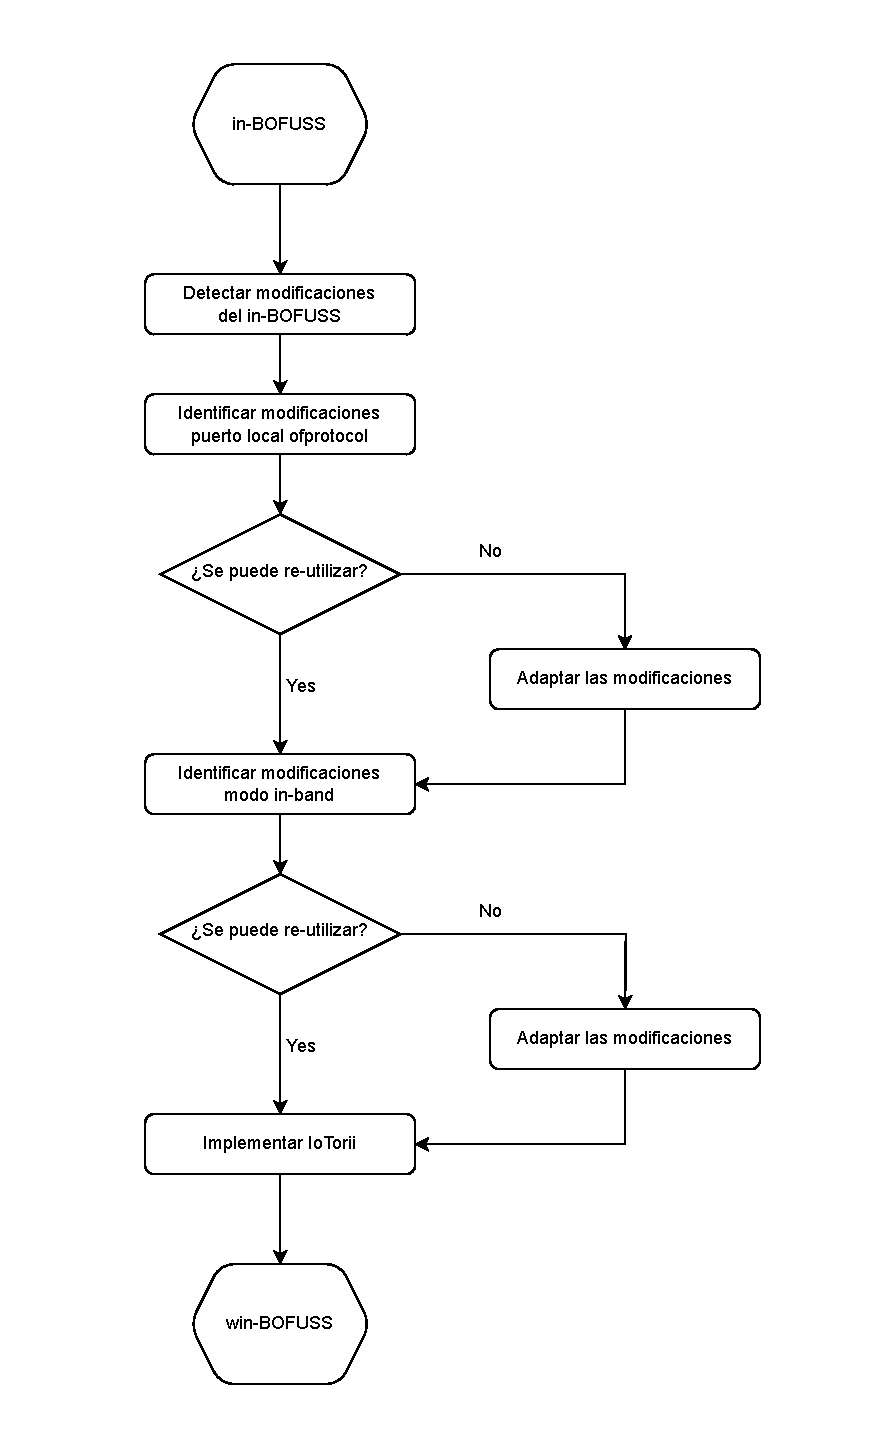
\includegraphics[width=0.75\textwidth]{archivos/img/dev/winBOFUSS.pdf}
    \caption{Diagrama de flujo para la implementación del protocolo IoTorii en el software switch \glsentryshort{bofus}}
    \label{fig:WIN-BOFUSS}
\end{figure}

\subsection{Implementación del protocolo IoTorii}

La implementación de IoTorii está basada en una publicación del grupo de investigación NetIS de la Universidad de Alcalá \cite{rojas2021outperforming}. El funcionamiento del protocolo está descrito en la Sección \ref{sec:ana_inband}, y con él conseguiremos crear múltiples caminos desde cualquier nodo de la topología al nodo raíz. La idea de utilizar este protocolo según se comentó es para tener caminos de respaldo en cada nodo hacia el nodo raíz, pudiendo conmutar de uno a otro cuando sea necesario, bien sea porque un equipo ha fallado o porque al ser un entorno inalámbrico donde la movilidad es intrinseca el \textit{next-hop} al nodo raíz ya no se encuentra en rango.\\
\\
En la Figura \ref{fig:iotoriiFulls}, se indica el diagrama de flujo con la implementación del protocolo en el \gls{bofus}. En primer lugar, al poner el switch en el modo de control in-band, se inicializa la lógica de IoTorii. Una vez que el protocolo IoTorii ha sido inicializado, el nodo raíz comienza la exploración, propagando los paquetes utilizados para generar los caminos que posteriormente serán almacenados en las tablas IoTorii de los nodos. Dichos paquetes, de tipo \textit{SetHLMAC}, solo serán entregados a los nodos que cumplan la condición de vecinos, es decir, aquellos nodos que hayan sido notificados mediante un mensaje de tipo \textit{Hello}. Cuando una ruta de la tabla HLMAC no se ve renovada, es decir, el nodo anexo al siguiente salto de esa ruta no ha enviado un mensaje de tipo \textit{Hello}, esta ruta se invalidará y se saltará a la siguiente dentro de la tabla HLMAC. Cuando esto ocurre el puerto local será el mismo, dado que la interfaz será la misma, pero el \textit{next-hop} no lo será dado que cambiará, habrá que actulizar la MAC destino en la conexión TCP que se realiza através de un mensaje netlink al stack de red del Kernel. \\
\\
En un entorno Linux, es posible utilizar Netlink para modificar la dirección MAC de destino asociada a una IP específica en la tabla ARP. Netlink es una interfaz de comunicación entre el espacio de usuario y el espacio de Kernel que permite realizar diversas operaciones relacionadas con la configuración de red. Lo primero que se tiene que llevar a cado en esta operación es abrir una conexión Netlink para comunicarse con el Kernel. Esto implica crear un socket Netlink y enlazarlo a un tipo de mensaje Netlink en específico. Acto seguido, se tiene que preparar el mensaje Netlink de tipo \texttt{RTM\_NEWNEIGH} (mensaje utilizado para manipular la caché ARP), y establecer los atributos del mensaje, configurando los atributos del mensaje para indicar la IP y la nueva dirección MAC destino a fijar. Enviar dicho mensaje y gestionar la confirmación del Kernel. De esta forma podremos actualizar de una ruta HLMAC a otra, pero lamentablemente no se ha conseguido hacer la operación de forma automática sin cerrar el socket por lo que será necesario volver a abrir el socket TCP con el controlador.\\
\\



\begin{figure}[ht!]
    \centering
    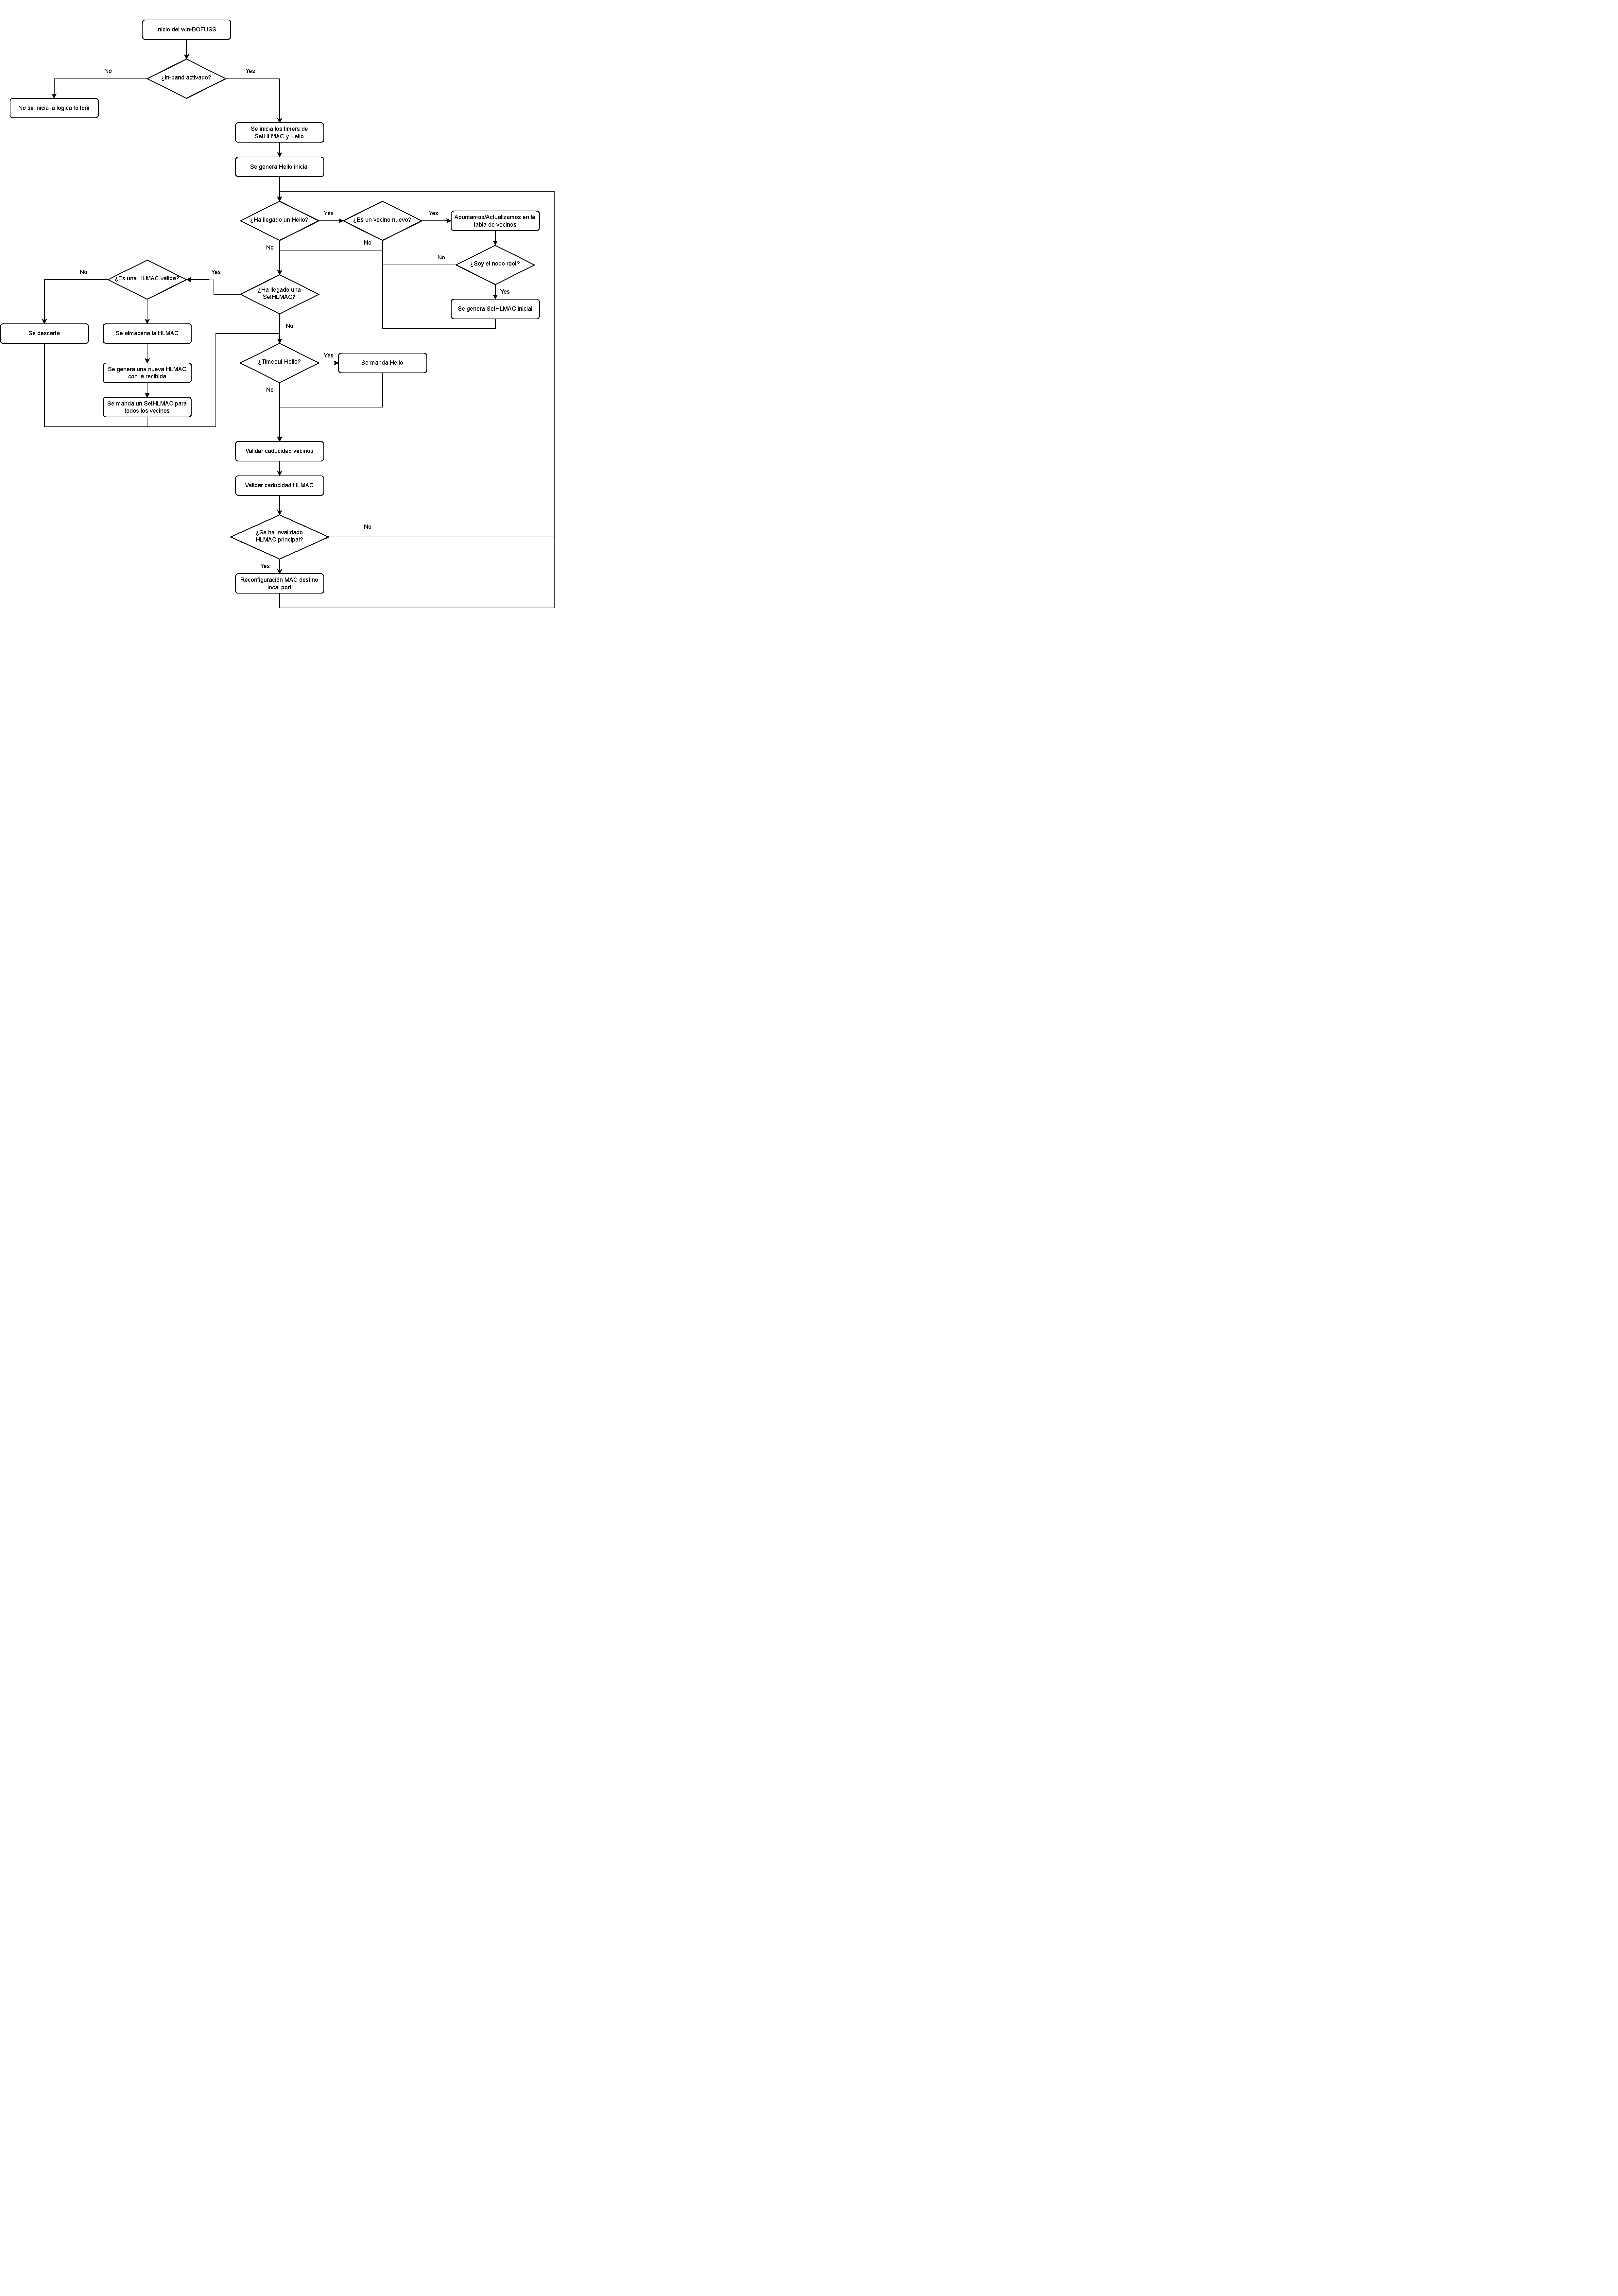
\includegraphics[width=\textwidth]{archivos/img/dev/iotorii.pdf}
    \caption{Diagrama de flujo de la operativa del protocolo IoTorii en el software switch \glsentryshort{bofus}}
    \label{fig:iotoriiFulls}
\end{figure}

\newpage

La importancia de establecer un temporizador para los mensajes \textit{Hello} y definir la caducidad de los vecinos en un protocolo radica en la mejora de su resiliencia y capacidad para adaptarse a cambios en la topología de la red. Estos mecanismos son fundamentales para mantener la conectividad y la estabilidad del protocolo en entornos dinámicos.\\
\\
El temporizador de los mensajes \textit{Hello} determina la frecuencia con la que los nodos del protocolo intercambian información de vecindad. Estos mensajes \textit{Hello} son vitales para conocer y mantener actualizada la lista de vecinos en la red. Al establecer un temporizador adecuado, se asegura que los nodos compartan regularmente información sobre su disponibilidad, estado y conexiones. Esto permite identificar rápidamente cambios en la topología de la red, como la caída de un enlace o la aparición de nuevos nodos. La caducidad de los vecinos define el tiempo que un nodo considera que un vecino sigue siendo alcanzable y activo. Cuando un vecino no responde a los mensajes \textit{Hello} dentro de este período, se considera que ha caducado y se elimina de la lista de vecinos. Establecer una caducidad adecuada es esencial para detectar y reaccionar rápidamente ante la pérdida de conectividad con un vecino. Al eliminar los vecinos caducados, se evita enviar tráfico a nodos inalcanzables y se garantiza que los recursos de red se utilicen de manera eficiente.\\
\\
La resilencia de un protocolo depende en gran medida de su capacidad para recuperarse rápidamente de fallos en la red y adaptarse a cambios en la topología. Al establecer un temporizador de mensajes \textit{Hello} y una caducidad de vecinos adecuados, el protocolo puede detectar y responder de manera oportuna a eventos como enlaces caídos, nodos inalcanzables o nuevos vecinos. Esto permite que el protocolo reconstruya rápidamente su tabla de vecinos y ajuste sus rutas en consecuencia, minimizando el impacto de las fallos y optimizando la utilización de los recursos de red.\\
\\
A continuación se van a indicar algunas de las modificaciones más importantes a la hora de implementar la lógica del protocolo IoTorii.

\begin{itemize}
    \item La estructura \texttt{reg\_HLMAC}, ha sido creada para representar una entrada de la tabla de HLMACs, también conocida como tabla de rutas de IoTorii. Cada entrada tiene almacenada la HLMAC, un flag de si está activa o no.
    \item La estructura \texttt{table\_HLMAC}, ha sido creada para representar la tabla de HLMACs, que viene a ser una lista enlazada simple de estructuras \texttt{reg\_HLMAC}.
    \item La estructura \texttt{reg\_nb}, ha sido creada para representar una entrada de la tabla de vecinos. Cada entrada tiene almacenada la MAC real del vecino, un flag de si está activa o no, y el sufijo único asignado.
    \item La estructura \texttt{table\_nb}, ha sido creada para representar la tabla de vecinos, que viene a ser también una lista enlazada simple de estructuras \texttt{reg\_nb}.
    \item Se ha adaptado la función \texttt{table\_AMACS\_add\_AMAC()} con las nuevas estructuras de datos, para que gestione el guardado de las HLMACs de IoTorii en vez de las AMACs. La función se ha renombrado a \texttt{table\_HLMACS\_add\_HLMAC()}.
    \item Se ha modificado la función \texttt{dp\_ports\_output\_amaru()}, la cual se encargaba de crear y enviar un paquete de Amaru por todas las interfaces del switch, para que ahora, dado que solo va a haber una interfaz genere los mensajes \textit{SetHLMAC} por la interfaz por los $N$ vecinos que tenga el nodo en cuestión. La función se ha renombrado a \texttt{dp\_ports\_output\_iotorii()}.
    \item Se han adaptado las funciones \texttt{disable\_invalid\_amacs\_UAH()} y \texttt{enable\_valid\_\\amacs\_UAH()}, las cuales se utilizaban para conmutar el \textit{flag} de active de las rutas, para que puedan trabajar con las nuevas estructuras de datos HLMAC. Las funciones se han renombrado a \texttt{disable\_invalid\_hlmacs\_UAH()} y \texttt{enable\_valid\_hlmacs\_UAH()} respectivamente.
    \item Se ha modificado la función \texttt{configure\_new\_local\_port\_amaru\_UAH()}, la cual se encargaba de buscar en la tabla de rutas AMACS, para que busque en la nueva tabla HLMAC y que aparte gestione el traspaso de una ruta a otra, modificando vía Netlink la nueva MAC destino del siguiente salto. La función se ha renombrado a \texttt{configure\_new\_local\_port\_iotorii\_UAH()}.
    \item Se ha modificado la función \texttt{send\_amaru\_new\_localport\_packet\_UAH()}, para que ajuste las reglas de las tablas de flujos del ofdatapath mediante una generación de un mensaje de tipo \texttt{PACKET\_IN} que se envía al ofprotocol.
    \item Se ha modificado la función \texttt{dp\_ports\_run()}, la cual de forma periorida verificará el estado del puerto, y además gestionará las funciones \texttt{disable\_invalid\_amacs\_UAH()} y \texttt{enable\_valid\_amacs\_UAH()} verificando la caducidad de las entradas. En caso de caducar una ruta activa se llamará a la función, \texttt{install\_new\_localport\_rules\_UAH()}, y a la función \texttt{configure\_new\_local\_port\_iotorii\_UAH()} para gestionar la instalación de una ruta alternativa.
    \item Se han creado una lógica de control de timer para la generación de los mensajes \textit{Hello}s. Toda la lógica está incluida en la función \texttt{timer\_UAH()}.
\end{itemize}